\documentclass[tikz,border=3pt]{standalone}
\usepackage[utf8]{inputenc}
\usepackage[T1]{fontenc}
\usepackage{lmodern}
\renewcommand{\familydefault}{\sfdefault}
\usepackage{sansmath}\sansmath
\usepackage{chemfig}
\usepackage{pgfplots}\pgfplotsset{compat=1.18,/pgf/number format/use comma,/pgf/number format/1000 sep={.}}
\usetikzlibrary{arrows.meta,calc,positioning,decorations.pathmorphing,patterns}
% paleta del sitio
\definecolor{nar}{HTML}{E8680C}\definecolor{narc}{HTML}{FFB35C}\definecolor{hielo}{HTML}{FFF3E8}
\definecolor{tinta}{HTML}{1D1D1F}\definecolor{gris}{HTML}{6E6E73}\definecolor{lila}{HTML}{7C5CF0}
\definecolor{azul}{HTML}{2F6FD6}\definecolor{menta}{HTML}{17A673}\definecolor{coral}{HTML}{E8342A}
\begin{document}
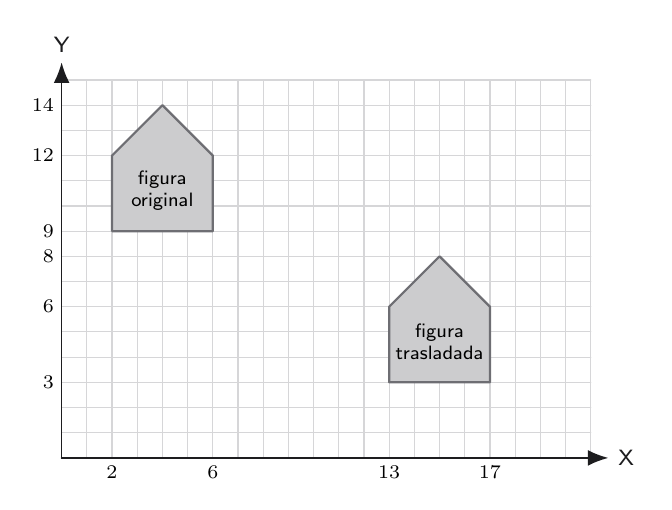
\begin{tikzpicture}[font=\small,x=0.32cm,y=0.32cm,line cap=round,line join=round,step={(1,1)}]
\draw[gris!28,thin] (0,0) grid (21,15);
\draw[-{Latex[length=2.6mm,width=2mm]},tinta,semithick] (0,0)--(21.7,0) node[right,font=\footnotesize] {X};
\draw[-{Latex[length=2.6mm,width=2mm]},tinta,semithick] (0,0)--(0,15.7) node[above,font=\footnotesize] {Y};
\node[below,font=\scriptsize,inner sep=1.5pt,fill=white,fill opacity=.85,text opacity=1] at (2,-0.12) {$2$};
\node[below,font=\scriptsize,inner sep=1.5pt,fill=white,fill opacity=.85,text opacity=1] at (6,-0.12) {$6$};
\node[below,font=\scriptsize,inner sep=1.5pt,fill=white,fill opacity=.85,text opacity=1] at (13,-0.12) {$13$};
\node[below,font=\scriptsize,inner sep=1.5pt,fill=white,fill opacity=.85,text opacity=1] at (17,-0.12) {$17$};
\node[left,font=\scriptsize,inner sep=1.5pt,fill=white,fill opacity=.85,text opacity=1] at (-0.12,3) {$3$};
\node[left,font=\scriptsize,inner sep=1.5pt,fill=white,fill opacity=.85,text opacity=1] at (-0.12,6) {$6$};
\node[left,font=\scriptsize,inner sep=1.5pt,fill=white,fill opacity=.85,text opacity=1] at (-0.12,8) {$8$};
\node[left,font=\scriptsize,inner sep=1.5pt,fill=white,fill opacity=.85,text opacity=1] at (-0.12,9) {$9$};
\node[left,font=\scriptsize,inner sep=1.5pt,fill=white,fill opacity=.85,text opacity=1] at (-0.12,12) {$12$};
\node[left,font=\scriptsize,inner sep=1.5pt,fill=white,fill opacity=.85,text opacity=1] at (-0.12,14) {$14$};
\filldraw[fill=gris!35,draw=gris,thick] (2,9)--(6,9)--(6,12)--(4,14)--(2,12)--cycle;
\filldraw[fill=gris!35,draw=gris,thick] (13,3)--(17,3)--(17,6)--(15,8)--(13,6)--cycle;
\node[font=\scriptsize,align=center] at (4,10.6) {figura\\original};
\node[font=\scriptsize,align=center] at (15,4.6) {figura\\trasladada};
\end{tikzpicture}
\end{document}
